\documentclass[11pt]{article}

\usepackage[utf8]{inputenc}
\usepackage[T1]{fontenc}
\usepackage{lmodern}
\usepackage[margin=1in]{geometry}
\usepackage{graphicx}
\usepackage{booktabs}
\usepackage{amsmath}
\usepackage{amssymb}
\usepackage{microtype}
\usepackage[hidelinks,pdfauthor={Bamdad Dashtban},pdftitle={Concept-Injection Introspection in Open Models Is Dose-Fragile}]{hyperref}

\setlength{\parskip}{0.5em}
\setlength{\parindent}{0pt}

\title{Concept-Injection Introspection in Open Models Is Dose-Fragile;\\
Its One Above-Chance Signal Does Not Replicate Across Scale}
\author{Bamdad Dashtban}
\date{}

\begin{document}
\maketitle

\begin{abstract}
We reproduce the concept-injection introspection protocol of Lindsey et al.\ (2025, ``Emergent Introspective Awareness in Large Language Models'') on open Qwen2.5 models. Two findings result. First, the effect is dose-fragile: an injection strength calibrated for coherent activation steering sits roughly 4 to 18 times below the paper's absolute strength, and at that under-dose every model returns a clean null that passes every sanity check (flat controls, a working positive control, coherent transcripts). Correcting the dose to the paper's regime and adding a fails-loud judge is what surfaces any signal at all. Second, at the corrected dose the picture is a null across the board with a single exception that does not generalize. Filling a base / general-instruct / code-instruct grid at 7B, 14B, and 32B, every rung scores 0/216 strict correct-identification except Qwen2.5-Coder-32B, which scores 2.3\% (5/216), above both a no-injection and a random-direction control with non-overlapping 95\% CIs. That one above-chance cell does not replicate down the Coder size ladder: Coder-7B is 0/216 and Coder-14B is 1/216 strict (two trials named the concept, one incoherent, so one passes the strict coherent-and-correct rule), both with CIs overlapping the 0.000 controls. The honest reading is a conjunction --- the signal appears only where code-heavy post-training meets $\sim$32B scale --- not a fine-tune main effect and not a scale main effect, and it rests on one marginal cell. Within the 32B row the base control still rules out parameter count (all three are 32B) and fine-tuning in general (Instruct is a fine-tune and is null), and a logit-lens localizes that cell's mechanism: the injected concept is linearly decodable at the unembedding in Coder-32B but not in base or Instruct, a legibility difference introduced by code-heavy post-training rather than suppression. We report the effect with the caveat that it is small, rests on a single a-priori dose, and does not survive its own size ladder. An earlier version of this note framed the 32B result as fine-tune-dependent rather than scale-dependent; the size ladder retracts that, since within the Coder family the effect is present only at 32B.
\end{abstract}

\section{Introduction}

Lindsey et al.\ inject a known concept vector into a model's residual stream and ask whether the model can report that an injected thought is present and name it. On frontier closed models the effect is real but unreliable. We ask a scaling question on open models: does this ability emerge with parameter count. The answer we reach is that no model from 7B to 32B shows robust detection, and the single above-chance cell we do find (Coder-32B) does not replicate down its own size ladder, so the signal is a conjunction of code-heavy post-training and $\sim$32B scale rather than a function of scale or fine-tune alone. Getting to that answer required first noticing that our own initial null was an artifact of dose calibration, which is a result in its own right for anyone trying to replicate this line of work.

Contributions: (1) a controllable, deterministic open-model reproduction with a fails-loud judge; (2) the dose-fragility result, with the exact under-dose that fakes a clean null; (3) a base/instruct/coder grid at 7B, 14B, and 32B showing that the one above-chance cell (Coder-32B) does not replicate across scale, so code post-training is at most necessary-but-not-sufficient; (4) a logit-lens that identifies the mechanism of that one cell as representational legibility.

\section{Method}

\textbf{Concept vectors.} Diff-of-means over concept-versus-baseline prompts (the paper's stated estimator), taken as a unit direction with its raw norm retained.

\textbf{Injection.} A forward hook adds the concept direction to the residual stream at depth 0.61, at strength $\alpha = 2 \cdot \|\text{raw diff-of-means}\|$ (the paper's canonical strength of 2). This is a single a-priori dose; we run no strength or layer sweep, so a positive cannot be an artifact of tuning to it. We log the applied magnitude ratio and cosine to confirm the injection is live rather than a no-op or a coherence-destroyer.

\textbf{Judge.} Detection is scored \texttt{coherent AND correct-identification} by Claude Sonnet 4 via AWS Bedrock, configured to raise on any parse error so a degraded or unavailable judge can never silently return a zero. Every transcript is persisted for offline re-judging.

\textbf{Controls.} Every point carries a no-injection control and a random-direction control matched to the concept vector's norm; detection counts only when the injected condition clears both. A positive control grades four canned responses through the real judge to prove it can emit a success and withholds it otherwise.

\section{Results}

\textbf{Corrected-dose Instruct ladder (Qwen2.5-Instruct, 216 trials per condition, seeds 0/1/2, one A100-80GB, fp16).} Correct-identification is 0.000 at every rung from 0.5B to 32B, with both controls flat at 0.000. The dose is live, not inert: at 32B the model affirms an injected thought 47\% of the time under injection versus never without it, and coherence climbs with scale (0.5\% coherent at 0.5B, 94\% at 32B). The models feel the perturbation; they do not name it.

\begin{figure}[htbp]
\centering
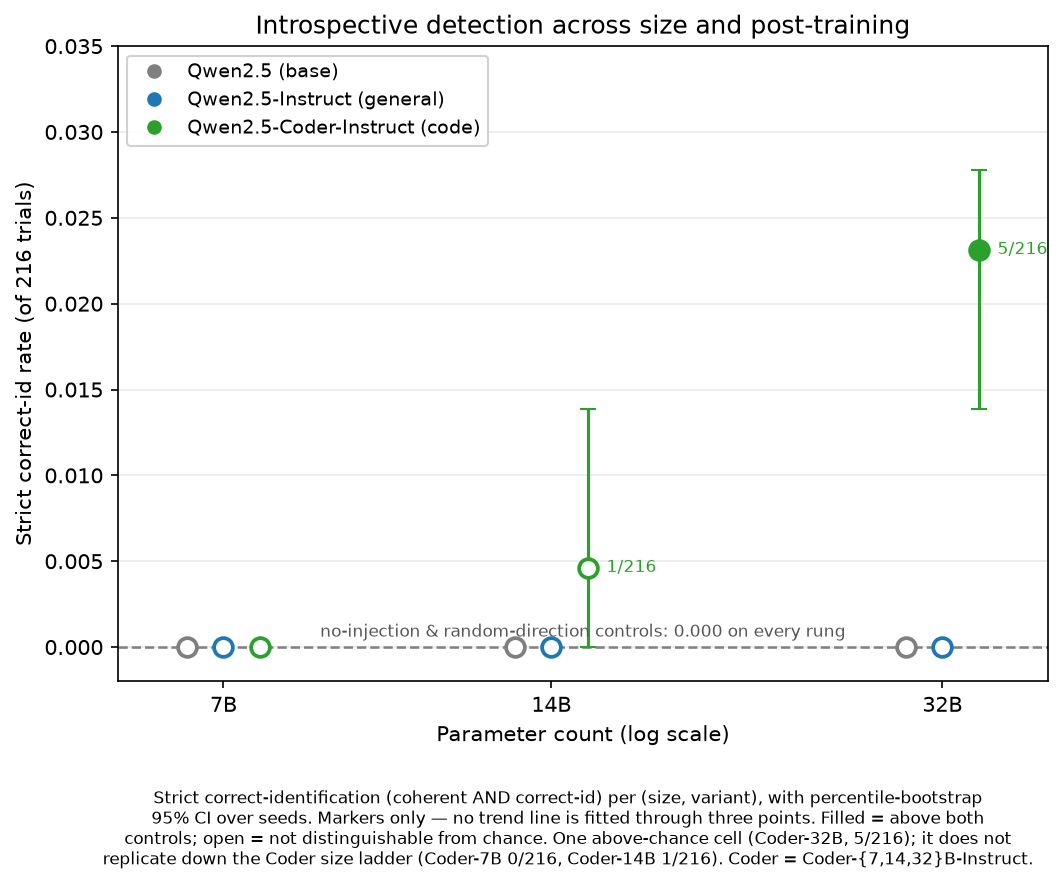
\includegraphics[width=0.85\linewidth]{../results/scaling_trend_k2.png}
\caption{Strict correct-identification per (size, variant) with percentile-bootstrap 95\% CI bars. Discrete markers, no fitted trend line. Every variant sits on the 0.000 floor at 7B and 14B; one Coder point lifts at 32B (filled $=$ above both controls). One above-chance cell (Coder-32B, 5/216); it does not replicate down the Coder size ladder (Coder-7B 0/216, Coder-14B 1/216). Coder $=$ Coder-\{7,14,32\}B-Instruct.}
\label{fig:scaling}
\end{figure}

\textbf{The 32B three-way (fixed size, fixed dose).}

\begin{table}[htbp]
\centering
\begin{tabular}{lcccc}
\toprule
Model (32B) & correct-id [95\% CI] & affirmative & coherent & above chance \\
\midrule
Qwen2.5-32B (base)   & 0.000 [0.000, 0.000] & 0.449 & 0.491 & no  \\
Qwen2.5-32B-Instruct & 0.000 [0.000, 0.000] & 0.472 & 0.944 & no  \\
Qwen2.5-Coder-32B    & 0.023 [0.014, 0.028] & 0.306 & 0.773 & yes \\
\bottomrule
\end{tabular}
\caption{The 32B three-way comparison: same parameter count, same dose, only post-training differs.}
\label{tab:threeway}
\end{table}

Base and Instruct sit at the floor and behave alike (they affirm around 45 to 47\% and never correctly identify). Only the code-tuned model lifts off. Within this 32B row the base rung is the control that matters: it removes parameter count (all three are 32B) and fine-tuning in general (Instruct is a null fine-tune) as explanations for \emph{this cell}. But the 32B row is not the whole story --- see the size ladder next.

\textbf{The size ladder (base and Coder at 7B, 14B, 32B, same dose and design).} Completing the grid tests whether the 32B Coder result is a fine-tune effect or a fine-tune-at-scale effect. It is the latter, weakly. \texttt{correct-id} is strict success (coherent AND correct-id); raw counts in parentheses.

\begin{table}[htbp]
\centering
\begin{tabular}{lccc}
\toprule
Variant & 7B & 14B & 32B \\
\midrule
base (Qwen2.5)                   & 0.000 (0/216) & 0.000 (0/216) & 0.000 (0/216) \\
general-instruct (-Instruct)     & 0.000 (0/216) & 0.000 (0/216) & 0.000 (0/216) \\
code-instruct (-Coder-Instruct)  & 0.000 (0/216) & 0.005 (1/216) & \textbf{0.023 (5/216)} \\
\bottomrule
\end{tabular}
\caption{The size ladder. Only the 32B Coder cell is above chance.}
\label{tab:ladder}
\end{table}

Only the 32B Coder cell is above chance. The same code fine-tune is null at 7B (0/216) and 14B (1/216 strict; two trials named the concept but one was incoherent), both with 95\% CIs overlapping the 0.000 controls. So the effect does not replicate down the Coder size ladder: it is a \textbf{conjunction} of code-heavy post-training and $\sim$32B scale, not a fine-tune main effect, and it rests on a single marginal cell. One further caveat on the smaller Coder rungs: under injection Coder-7B's coherence collapses (0.972 to 0.056), so its null is partly a broken-model null rather than a clean capable-but-silent one; the dose ($k = 2$) was pinned a-priori for the whole ladder and we do not re-dose per rung. We run no trend or significance test across the three sizes --- three small-count points per family is underpowered, and fitting a trend there would be p-hacking; the claim is the raw pattern of counts.

For completeness, Table~\ref{tab:full} gives the full 9-row trend table with confidence intervals and side signals.

\begin{table}[htbp]
\centering
\small
\begin{tabular}{llccccc}
\toprule
Model & Variant & correct-id (x/216) [95\% CI] & affirm. & coher. & above chance? \\
\midrule
Qwen2.5-7B            & base     & 0.000 (0/216) [0.000, 0.000]          & 0.204 & 0.218 & no      \\
Qwen2.5-7B-Instruct   & instruct & 0.000 (0/216) [0.000, 0.000]          & 0.306 & 0.597 & no      \\
Qwen2.5-Coder-7B      & coder    & 0.000 (0/216) [0.000, 0.000]          & 0.310 & 0.056 & no      \\
Qwen2.5-14B           & base     & 0.000 (0/216) [0.000, 0.000]          & 0.074 & 0.412 & no      \\
Qwen2.5-14B-Instruct  & instruct & 0.000 (0/216) [0.000, 0.000]          & 0.023 & 0.894 & no      \\
Qwen2.5-Coder-14B     & coder    & 0.005 (1/216) [0.000, 0.014]          & 0.093 & 0.509 & no      \\
Qwen2.5-32B           & base     & 0.000 (0/216) [0.000, 0.000]          & 0.449 & 0.491 & no      \\
Qwen2.5-32B-Instruct  & instruct & 0.000 (0/216) [0.000, 0.000]          & 0.472 & 0.944 & no      \\
Qwen2.5-Coder-32B     & coder    & \textbf{0.023 (5/216)} [0.014, 0.028] & 0.306 & 0.773 & \textbf{yes} \\
\bottomrule
\end{tabular}
\caption{Full trend table. Each cell is 216 trials (6 concepts $\times$ 12 trials $\times$ 3 seeds). ``Coder'' $=$ Qwen2.5-Coder-\{7,14,32\}B-Instruct. Both controls (no-injection, random-matched) are 0.000 on every rung, so only the injected column is shown.}
\label{tab:full}
\end{table}

\textbf{Mechanism (logit-lens).} Projecting the injected residual through the model's own unembedding, injection sharply raises the injected concept token in Coder-32B (median rank about 30k to 4k, a sustained lift of roughly 2 to 2.5 over no injection, several concepts reaching the top few). In Instruct-32B and base the concept stays illegible: rank no better than no injection, worse than a matched-random direction. The dissociation is a legibility difference from post-training, not a persona gate, which matches the behavioural signature of affirming a thought while naming the wrong one.

\section{The dose-fragility result}

Our first pass reported a clean null on every model, including Coder-32B where the effect is claimed. It was wrong for two compounding reasons. The injection dose was inherited from a companion steering study and tuned for coherent output, which put it roughly 4 to 18 times below the paper's absolute strength; the effect-size measurement, not the detection score, is what exposed this. Separately, a same-day judge-API credit outage silently turned grades into false negatives. Correcting the dose to the paper's regime and moving to a fails-loud judge is what surfaced the real signal. We keep the superseded numbers in the repository, marked, because the wrong turn is half the story: a steering-calibrated dose plus a quiet judge will hand you a null you will believe.

Dose-fragility has a second face that is cross-model, not just cross-strength. Taking the same norm-relative $k = 2$ dose out of the Qwen family to DeepSeek-Coder-33B-Instruct --- correctly proportioned to that model's own residual norm ($\alpha = 2 \cdot \|\text{raw diff-of-means}\| = 899$, magnitude-ratio 1.02) and not over-dosed --- collapses coherence: injected coherent 0.042 and random-direction 0.093 against 1.000 with no injection, transcripts reduced to word-salad, correct-id 0/216 strict. The tell is that the random-direction control collapses \emph{alongside} the injected condition (0.093): if the concept direction were the cause, the injected condition would fall while the matched-norm control held. Both falling together means the dose magnitude, not the injected concept, broke the model --- so this 0/216 is a \textbf{broken-model null}, an invalid test rather than evidence about introspection, the same failure mode as Coder-7B (0.972 $\to$ 0.056) reproduced in a different model family. The identical dose leaves Qwen2.5-Coder-32B (0.773 coherent), the Qwen1.5-MoE probe (\S\ref{sec:moe}, 0.750), and the dense Qwen rungs intact, so coherence tolerance to a correctly-proportioned dose is model-specific: a matched norm-relative strength that is coherent on some models destroys it on others. This changes nothing in the headline --- Coder-32B remains the single above-chance cell and this rung enters nothing into it; we log it for transparency (records and judged transcripts committed, \texttt{33ba9d2}). A second out-of-family rung, \textbf{CodeLlama-34B-Instruct}, reproduces the same collapse at the identical dose (injected coherent 0.056, random-direction 0.060, against 1.000 with no injection; correct-id 0/216 strict; word-salad transcripts; committed \texttt{6e21a89}). So the pattern is a three-versus-three split: the pinned norm-relative dose collapses coherence on Coder-7B, DeepSeek-33B, and CodeLlama-34B, while it stays coherent on Coder-32B (0.773), the Qwen1.5-MoE probe (\S\ref{sec:moe}, 0.750), and the dense Qwen rungs. It carries one methods lesson, and it is \emph{not} about generation length. A cheap pre-run coherence gate passed on both DeepSeek-33B and CodeLlama-34B, yet the Bedrock-judged runs collapsed; on \emph{identical} transcripts the gate's rule-based coherence proxy rated 0.79--0.89 coherent while the authoritative Bedrock judge rated 0.04--0.06. The proxy is simply too lenient and waves through word-salad --- length is ruled out because CodeLlama's gate already sampled at the full 200-token scoring length and still passed. A coherence gate must be scored by the same judge as the trials it protects; a Bedrock-judged gate is the obvious future-work fix.

\section{Generalization: a cross-architecture (MoE) probe}
\label{sec:moe}

\textbf{State the confound before the result.} The cross-architecture probe runs the same concept-injection protocol on a \textbf{mixture-of-experts} model, \textbf{Qwen1.5-MoE-A2.7B-Chat} (\textbf{2.7B active / 14.3B total, 24 layers}), a general-instruct MoE. That model sits \textbf{far below the $\sim$32B-active scale} where the one above-chance cell appeared, \textbf{and} it carries \textbf{no code-specific post-training}. On both axes that made the Coder-32B cell light up (code-heavy post-training AND $\sim$32B scale), this MoE is on the \emph{null} side --- it is the architectural analog of our dense general-instruct arm, which is null at every size we tested. So a null here is \textbf{predetermined by scale and post-training, not by architecture}; it is not a verdict that ``MoE models cannot introspect.'' The probe is not run to see whether an MoE ``passes.'' It has two narrower, honest jobs.

\textbf{STEP 1 --- is the injection hook live on MoE expert routing?} The injection is a \texttt{repeng.ControlModel} forward hook, and \texttt{repeng} assumes a mistral/Qwen-shaped \texttt{model.model.layers} stack. An MoE decoder layer routes through experts and its \texttt{forward} can return a \texttt{(hidden, router\_logits)} tuple, so the hook can attach to the wrong tensor and \textbf{silently no-op} --- scoring a clean but meaningless null. STEP 1 requires a live perturbation before anything else counts, and it passed: the stack resolved via \texttt{model.model.layers}, and the injected direction is live, correctly oriented, and \textbf{demonstrably changes expert routing}.

\begin{table}[htbp]
\centering
\begin{tabular}{lc}
\toprule
STEP-1 gate (Qwen1.5-MoE-A2.7B-Chat) & value \\
\midrule
injection layer (depth 0.61 of 24)              & 15 \\
dose $\alpha = 2 \times \text{raw\_norm}$ (4.447) & 8.893 \\
magnitude ratio (live if $\gg 0$)               & 1.061 \\
cosine to intended direction                    & 0.885 \\
\textbf{routing changed} (top-$k$ expert set flips) & \textbf{0.786} of MoE positions \\
expert-gate L1 shift / MoE positions            & 0.312 / 1422 \\
\bottomrule
\end{tabular}
\caption{STEP-1 fit-check: the residual-injection hook is live on the MoE and perturbs expert routing.}
\label{tab:moe-step1}
\end{table}

The \texttt{routing\_changed} $= 0.786$ is the load-bearing number: the top-$k$ expert \emph{set} flips at 79\% of positions under injection, so the hook perturbs expert \emph{selection} and writes to the real post-expert residual, not a discarded copy. The silent-no-op failure mode is ruled out. These STEP-1 numbers are the committed fit-check artifact (\texttt{results/moe\_fitcheck.json}); regenerate with \texttt{modal run modal\_app.py::moe\_fitcheck}.

\textbf{STEP 2 --- a same-scale dense-parity check.} With the hook proven live, STEP 2 asks whether the MoE sits on the dense null curve at its own active scale. It does.

\begin{table}[htbp]
\centering
\small
\begin{tabular}{lccccc}
\toprule
Model (MoE, 2.7B active / 14.3B total) & correct-id (x/216) [95\% CI] & affirmative & coherent & above chance? \\
\midrule
Qwen1.5-MoE-A2.7B-Chat & 0.000 (0/216) [0.000, 0.000] & 0.005 (1/216) & 0.750 & \textbf{no} \\
\bottomrule
\end{tabular}
\caption{STEP-2 dense-parity check. The MoE sits on the dense null curve at its own active scale.}
\label{tab:moe-step2}
\end{table}

Both controls (no-injection, random-direction) are 0.000 on correct-id. Coherence by condition: no-injection 0.931, injected 0.750, random-direction 0.648. Read this carefully, and do not over-read it in either direction. \textbf{The headline is a mechanism/behaviour dissociation:} the injection is mechanistically live (79\% of positions re-route, magnitude ratio $\sim$1.06) and yet produces \textbf{zero introspective detection} (0/216, not above chance) --- the same null as the dense sub-32B rungs, so a small general-instruct MoE sits \textbf{on} the dense null curve, not off it. \textbf{The near-floor affirmative (0.005) is a scale fact, not an architecture break:} the strong ``affirms an injected thought $\sim$45\%'' signature was scale-dependent in the dense models too --- 32B affirms $\sim$45\%, but 14B-Instruct affirms only 0.023 (5/216) --- so a floor affirmative at 2.7B active is what small \emph{dense} models do, attributable to scale, not to MoE architecture. We report the number and do not claim a dissociation the data cannot isolate. \textbf{And it is a genuine null, not a broken-model null:} coherence holds at 0.750 under injection (vs 0.931 without), so the model is largely capable-but-silent, unlike Coder-7B whose 0/216 was confounded by a coherence collapse to 0.056.

The publishable positive is STEP 1 as a methods result: the residual-injection hook transfers cleanly to an expert-routed architecture and demonstrably perturbs routing (79\% expert-set change), so the technique is not dense-only. The behavioural effect stays absent exactly as predetermined --- detection needed the conjunction of code-heavy post-training AND $\sim$32B scale, and this model has neither, so its null is \textbf{not an architecture verdict}. Whether a large-active, code-post-trained MoE (Kimi-K2 scale) would introspect is left open and estimated separately (see the K2 cost/feasibility estimate in \texttt{k2\_estimate.md}, gated on its own STEP-1 router-shift check).

\section{Limitations}

The Coder-32B effect is 2.3\%, modest, rests on a single a-priori dose with no sweep, and is the only above-chance cell in the whole 3-variant by 3-size grid --- it does not replicate at 7B or 14B of the same Coder fine-tune, so read it as at most necessary-but-not-sufficient evidence for code post-training. The non-replication is itself imperfect: Coder-7B's null is confounded by an injection-induced coherence collapse. We identify the 32B cell's mechanism as legibility but not its cause: we do not yet know which layers or features code post-training changes, or whether the driver is code specifically or a correlate of it. The cross-architecture MoE probe (\S\ref{sec:moe}) is now done --- the null it returns is predetermined by scale and post-training, not an architecture verdict; a 72B dense triple and a large-active code-post-trained MoE (K2-scale) remain the obvious next tests. Everything is fp16 on a single A100, dense Qwen only apart from that one MoE probe.

\section{Reproducibility}

Deterministic, fixed seeds (0/1/2), one Modal A100-80GB, fp16, corrected dose $\alpha = 2 \cdot \|\text{raw diff-of-means}\|$, Bedrock Sonnet 4 judge that fails loud. Total spend about 23 USD: roughly 6.6 USD in GPU (per-rung A100-80GB fp16, e.g.\ the 7B base rung was 0.55 USD) and about 16 USD in Bedrock judge calls. Code, raw transcripts, and the exact dose calibration are in the repository; a companion write-up is at \url{https://bamdad.substack.com/p/same-size-different-mind}.

\section*{Related work}
\addcontentsline{toc}{section}{Related work}

Lindsey et al., ``Emergent Introspective Awareness in Large Language Models'' (Anthropic, 2025; arXiv:2601.01828), the protocol we reproduce. Prior open-model replications on Qwen and Llama report the effect on code-tuned checkpoints; our base control and logit-lens give a mechanism for why those checkpoints and not their instruct siblings.

\begin{thebibliography}{1}
\bibitem{lindsey2025}
J.~Lindsey et al.,
``Emergent Introspective Awareness in Large Language Models,''
Anthropic, 2025. arXiv:2601.01828.
\end{thebibliography}

\end{document}
